\section{Angular Momentum}

\subsection{Orbital angular momentum}

\subsubsection{Classical orbital angular momentum}

\begin{wrapfigure}{r}{0.5\textwidth}
  \centering
  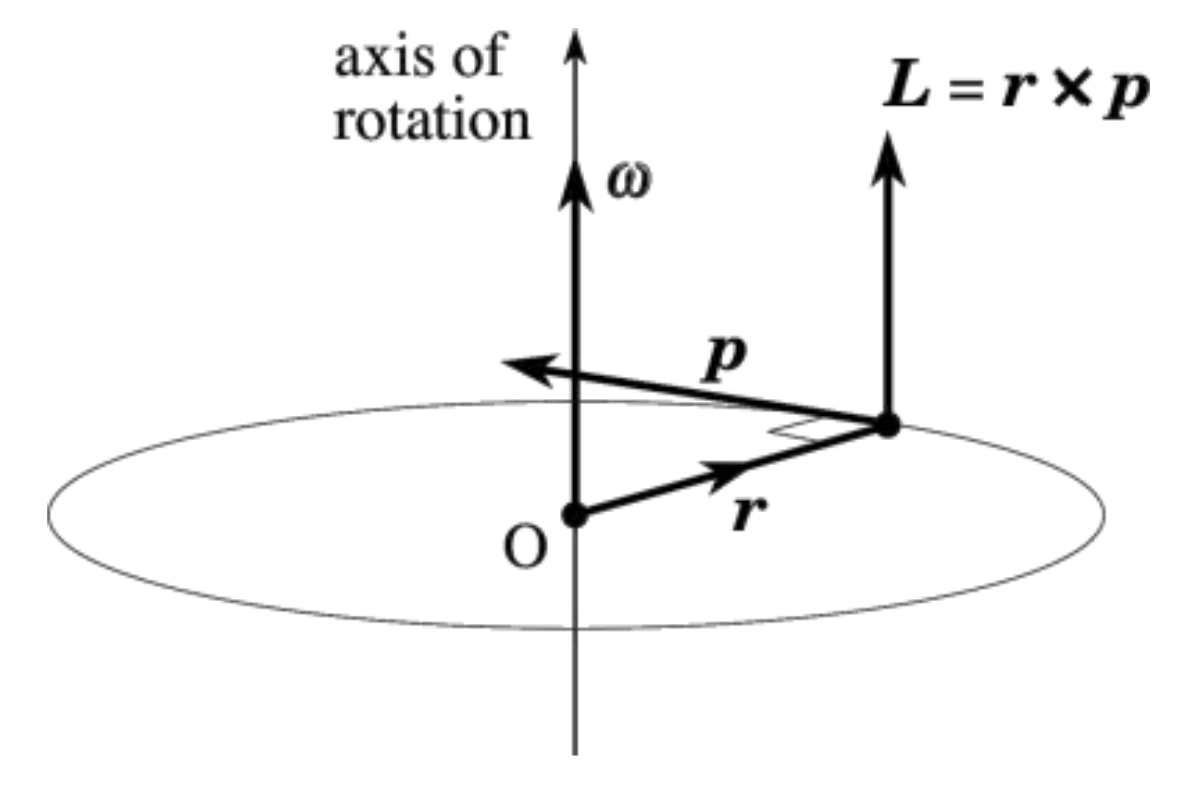
\includegraphics[width=0.5\textwidth]{images/classical_angular_momentum.png}
  \caption{Classical orbital angular momentum}
  \label{fig:classical_angular_momentum}
\end{wrapfigure}

In classical mechanics, the angular momentum of a particle relative to some axis is defined as:

\begin{equation}
    \vec{L} = \vec{r} \times \vec{p}
\end{equation}

where $\vec{r}$ is the position vector of the particle with respect to a point on the axis of rotation and $\vec{p}$ is its momentum. 

The total angular momentum of a system of particles is the sum of angular momenta of the individual particles:
\begin{equation}
    \vec{L}_\text{total} = \sum_i \vec{r}_i \times \vec{p}_i
\end{equation}

The total angular momentum varies in time according to the net external torque, which we can obtain by differentiating the total angular momentum with respect to time:
\begin{equation}
    \vec{\tau}_\text{total} = \sum_i \vec{\tau}_{\text{ext},i} = \frac{d\vec{L}_\text{total}}{dt}
\end{equation}

It follows that the total angular momentum of a system is conserved if the resultant external torque acting on the system is zero.

\subsubsection{Orbital angular momentum in quantum mechanics}

As discussed in \textbf{Section \ref{observables_and_operators}}, to obtain the quantum mechanical operator for orbital angular momentum from its classical definition, we can apply quantization to the classical expression provided in the previous section:
\begin{equation}
    \vec{L} = \vec{R} \times \vec{P} = -i\hbar \vec{R}\times \vec{\nabla}
\end{equation}

For a system of (spin-less) particles, the total angular momentum is defined as:
\begin{equation}
    \vec{L}_\text{total} = \sum_i \vec{R}_i \times \vec{P}_i
\end{equation}

The different cartesian components of the angular momentum operator are:
\begin{equation}
    \begin{split}
        L_x &= YP_z - ZP_y = -i\hbar \left(Y\frac{\partial}{\partial z} - Z\frac{\partial}{\partial y}\right) \\
        L_y &= ZP_x - XP_z = -i\hbar \left(Z\frac{\partial}{\partial x} - X\frac{\partial}{\partial z}\right) \\
        L_z &= XP_y - YP_x = -i\hbar \left(X\frac{\partial}{\partial y} - Y\frac{\partial}{\partial x}\right)
    \end{split}
\end{equation}
We can also define the square of the angular momentum operator:
\begin{equation}
    L^2 = L_x^2 + L_y^2 + L_z^2
\end{equation}
As expected from operators corresponding to observables, all angular momentum operators are Hermitian.

\subsubsection{Commutation relations}
